% Tool-Existence Hallucination Is Rarer Than Reported on BFCL Multi-Turn
% SCALE @ ICML 2026 — anonymous double-blind submission

\documentclass{article}

% Recommended ICML 2026 packages
\usepackage{microtype}
\usepackage{graphicx}
\usepackage{subcaption}
\usepackage{booktabs}
\usepackage{hyperref}
\usepackage{xurl}  % allow long URLs to break across lines in references
\newcommand{\theHalgorithm}{\arabic{algorithm}}

% Blind submission: \usepackage{icml2026}
% arXiv preprint: \usepackage[preprint]{icml2026}
% Camera-ready:   \usepackage[accepted]{icml2026}
\usepackage{icml2026}

\usepackage{amsmath}
\usepackage{amssymb}
\usepackage{mathtools}
\usepackage{listings}
\usepackage{xcolor}

% Listings setup for the RVR pseudocode in §3.
\lstset{
    basicstyle=\ttfamily\small,
    breaklines=true,
    showstringspaces=false,
    columns=fullflexible,
    frame=single,
    framerule=0.4pt,
    aboveskip=0.5em,
    belowskip=0.5em,
}

\icmltitlerunning{Tier-Dependent Tool-Existence Hallucination}

\begin{document}

\twocolumn[
\icmltitle{Tool-Existence Hallucination Is Tier-Dependent and \\
           Intra-Family Non-Monotonic on BFCL Multi-Turn}

\icmlsetsymbol{equal}{*}

\begin{icmlauthorlist}
\icmlauthor{Anonymous}{anon}
\end{icmlauthorlist}
\icmlaffiliation{anon}{~}

\icmlkeywords{tool-using agents, hallucination, function calling,
              BFCL, agent benchmarks, ICML 2026 SCALE}
\vskip 0.3in
]

% Suppress the icml2026.sty boilerplate "Anonymous Institution, City,
% Region, Country. Correspondence to: Anonymous Author <anon@...>".
\makeatletter
\renewcommand{\printAffiliationsAndNotice}[1]{\global\icml@noticeprintedtrue}
\makeatother
\printAffiliationsAndNotice{}

\begin{abstract}
Tool-name hallucination is a known failure mode. Who actually does it,
how often, and what fixes it? We define a per-call Tool-Existence
Hallucination Rate (TEHR) and run it on BFCL multi-turn against two
populations: five Anthropic 4.x versions across an eleven-month release
window, and the Qwen3-Instruct family at six sizes from $0.6$B to $32$B
(4-bit MLX). The Anthropic side is quiet. Across $2{,}599$
opaque-baseline calls we logged zero TEHR events, Clopper--Pearson 95\%
upper bound $\leq\!0.115\%$. Qwen3 isn't: its rate is non-monotone in
scale, climbing from $0\%$ at $0.6$B to $\mathbf{1.87\%}$ at $14$B and
back to $0\%$ at $32$B. We propose Registry-Visible Reprompting (RVR), a
training-free middleware that, on a registry miss, returns one re-prompt
wrapping a structured \texttt{tool\_not\_found} envelope. RVR removes all
fourteen pooled Qwen3 fabrications (Fisher's exact one-sided,
$p=7.1\!\times\!10^{-5}$ on $14/973$ vs.\ $0/945$). The surprise is where
the fix lives. An ablation that keeps the envelope but drops the registry
listing ($\mathrm{C}_{0.7}$; $0/253$ on Qwen3-8B) already hits zero, and a
decoy that fills the envelope with \emph{wrong} tool names
($\mathrm{C}_{0.8}$) does not re-introduce
fabrications\footnote{The decoy arm logs zero TEHR across all high-yield
Qwen3 conditions ($0/321$ pooled: near\_name $0/97$, synonym $0/106$,
matched\_random $0/107$), matching $\mathrm{C}_{0.7}$ ($0/253$) and the
real list $\mathrm{C}_1$ ($0/258$); registry content is decorative for
recovery.}. The recovery is format, not content: a single structured
rejection re-grounds the model regardless of what the registry says,
echoing the format-over-content effect Min et al.\ found for in-context
demonstrations~\citep{min2022rethinking}. Read this way, the mid-scale
bump stops being noise and becomes a predicted signature --- a U-shaped
capability window~\citep{wei2022ushaped,mckenzie2023inversescaling} in
the generative tool-name prior, controlled for quantization by the
$0$-and-$32$B endpoints that bracket it at the same 4-bit precision. On
Anthropic's zero-event regime RVR also logs zero, but the strict-pass
subset slips at $N\!=\!60$; we recommend tier-conditional deployment. Our
read: reactive agent error-recovery is less about telling the model the
right answer than about re-grounding its output format, and one
structured reply does it on the models where the failure shows up.
\end{abstract}

\section{Introduction}
\label{sec:intro}

An agent calls \texttt{search\_flights}. The registry contains
\texttt{find\_flights}. The call fails. Practitioners hit this
mismatch in production with Claude, Gemini, and Grok~\citep{czapla2026},
and what stings is that the model knew the task, picked something
plausible, and just got the name wrong. Existing benchmarks measure
related quantities at the wrong grain.
API-Bank~\citep{li2023apibank} reports per-task name-mismatch up to
$61.4\%$ on a 2023-vintage model set;
MetaTool~\citep{huang2024metatool} isolates fabrication via target
removal and scores per-query Correct Selection Rate on single-turn
prompts; RelyToolBench~\citep{cao2025reliability} folds
non-existent-tool invocations into a composite reliability number.
Read together, the failure looks architecture-agnostic and uniform.

We don't think it is. We define per-call \emph{Tool-Existence
Hallucination Rate} (TEHR) and run it over two populations on BFCL
multi-turn: the Anthropic 4.x family at five versions spanning
May~2025 to April~2026 (Opus~4.7, Sonnet 4/4.5/4.6, Haiku~4.5), and
Qwen3-Instruct at six sizes ($0.6$B--$32$B) in 4-bit MLX on
consumer hardware. Both see three BFCL splits plus a four-distractor
probe with the real target removed and a synthetic look-alike in
its slot. BFCL is strictly typed, so this isn't production, but it
is the closest we could get to Czapla's setting on a benchmark.
Figure~\ref{fig:scaling} is the headline.

The two families don't look alike. Across $2{,}599$ Anthropic calls
under $\mathrm{C}_0$, zero TEHR events (Clopper--Pearson 95\% upper
bound $\leq\!0.115\%$); the $\mathrm{C}_1$ subset adds $0/678$ at
$\leq\!0.441\%$. The split designed to coax fabrication,
\texttt{multi\_turn\_miss\_func}, didn't bite: the agent chained
five smaller in-registry calls instead of inventing a one-shot.
With every Anthropic cell at $0/N$, no temporal slope is fittable;
the five versions function as a stability check, not a trend.

Qwen3 looks nothing like that. Pooled per-call rates climb from
$0\%$ at $0.6$B through $0.95\%$, $1.33\%$, $1.49\%$, peak at
$\mathbf{1.87\%}$ at $14$B, and drop back to $0\%$ at $32$B
($N\!=\!224$, consistent with any true rate $\leq\!1.34\%$). Six
points isn't a curve. The \emph{type} of distractor that wins also
moves: $1.7$B peaks on near-name ($3.7\%$); $4$B/$8$B on
matched-random ($5.4\%$, $3.0\%$); $14$B on synonym ($7.2\%$). The
arc is consistent with a capability-sweet-spot story at $n\!=\!6$,
without confirming it; \citet{mckenzie2023inversescaling} report
similarly shaped non-monotonicities. A cross-family release covering
six additional open models is in the supplement.

Registry-Visible Reprompting (RVR) is what we built to fix this.
The middleware is training-free: intercept the proposed call, check
the name, and on a miss re-prompt with a structured
\texttt{tool\_not\_found} envelope listing what is available. Across
the four Qwen3 tiers with non-zero TEHR ($1.7$B, $4$B, $8$B, $14$B),
RVR clears all fourteen pooled fabrications: Fisher's exact one-sided
on $14/973$ vs.\ $0/945$ gives $p=7.1\!\times\!10^{-5}$. A
content-matched ablation ($\mathrm{C}_{0.7}$, $0/253$ on Qwen3-8B),
keeping the envelope structure but dropping the registry list, also
hits zero. The envelope is doing the work, not the listed names;
this surprised us. On the Anthropic zero-event regime RVR holds at
zero, but strict-pass slips (Sonnet $60\!\to\!53/60$; Haiku
$60\!\to\!56/60$); a Newcombe-hybrid TOST at $N\!=\!60$ is
underpowered for a $5$-pp non-inferiority margin, so we can't rule
the cost in or out. We argue for tier-conditional deployment.

The Anthropic $\mathrm{C}_0$ bound ($\leq\!0.115\%$ at $N=2{,}599$)
sits an order of magnitude below the Qwen3 point estimates in the
$0.95$--$1.87\%$ band. The bound-vs-estimate asymmetry is the
finding. The intra-family non-monotonic shape on Qwen3 is itself
descriptive evidence aggregate metrics couldn't have surfaced. We
release four artifacts: the per-call TEHR diagnostic, an
eleven-model audit over eleven months, RVR with per-tier validation,
and an open-source harness with $144$ unit tests. Total API spend
\$$73$; the Qwen3 sweep ran at zero marginal cost on the M5.

\section{Related Work}
\label{sec:related}

\paragraph{Tool-using agents and benchmarks.}
Tool-using LLM agents are evaluated on a small, fairly stable set of
suites. The Berkeley Function-Calling Leaderboard~\citep{bfcl2024,bfclv4_2025}
started as single-turn API selection and has grown into a stateful
multi-turn suite. $\tau$-bench~\citep{taubench2024} pushes in a different
direction, scoring dialog-driven retail and airline agents that must
reconcile a user goal against a tool catalog. Both report
\emph{end-to-end task success}, which fuses tool selection with reasoning,
parsing, and policy errors into one number. Trace-level harnesses
\citep{appworld2024,reactagent2023} expose more, yet still report
pass-rate as the headline. This is the wrong granularity for the
failure we care about; TFR isolates a portable slice of it across
vendors and benchmarks.

\paragraph{Empirical analysis of agent failures.}
Practitioners have informally reported that frontier models call tools
that were never declared. \citet{czapla2026} reproduces the behavior
across Claude, Gemini, and Grok, noting that ``Claude 4.5 hallucinated
access to a tool I hadn't given it yet \ldots I've reproduced similar
behavior with Gemini and Grok.'' On the academic side,
\citet{bugstudy2026} mine 998 bug reports from CrewAI and LangChain
and find ``API misuse,'' ``API incompatibility,'' and ``Documentation
Desync'' dominating the root-cause distribution, with the Self-Action
lifecycle stage hit hardest. Neither line puts a number on the failure
under controlled conditions. We do, formalizing the unauthorized-tool
subclass as TFR and reporting it across five models.

\paragraph{Prior tool-hallucination metrics.}
Tool-call name errors have been measured under several aggregations,
and the choice of denominator matters. \citet{li2023apibank} introduce
``API Hallucination'' in API-Bank as a ground-truth-vs-prediction
name-mismatch error category, with per-task error rates up to $61.4\%$
on then-current models. The closest prior measurement to ours is
\citet{huang2024metatool}, whose MetaTool sub-task~3 deliberately
removes the correct tool from the registry and tracks the resulting
fabrication through a per-query Correct Selection Rate. That isolates the
registry-membership phenomenon, but stays at the per-query
level on single-turn instructions. \citet{cao2025reliability} name the
phenomenon directly (``tool type hallucination,'' where the model
fabricates a tool absent from the available set), but their fix is a
training-time \emph{reliability alignment} that expands the action space
(defer / clarify / switch), and they report it inside a composite
reliability score rather than as a standalone per-call rate. We share
their target failure but differ on both axes: a per-call rate, and a
training-free inference-time intervention. The ``does the called tool
exist'' question is not itself new: ToolBeHonest~\citep{toolbehonest2024}
catalogues a \emph{non-existent tool} error category qualitatively, and
BFCL v4's hallucination metric \citep{bfclv4_2025} measures a different
failure, invoking a tool when none is appropriate. What is new is the
per-call operationalization across capability tiers and vendors, and the
content-controlled ablation (Section~\ref{sec:mechanism}) it makes
possible: TFR extends MetaTool's premise from \emph{per-query} to
\emph{per-call} on multi-turn agentic traces, and from controlled
removal to the natural distribution of registry-membership violations.
Per-call is what lets the intervention in Section~\ref{sec:method:rvr}
be evaluated against a content-controlled $C_{0.7}$ baseline, a contrast
aggregate metrics cannot expose. Appendix Table~\ref{tab:priorart}
positions TFR against these prior measurements by what each one counts;
the denominators and elicitation setups differ, so the numbers are not
directly comparable, but the granularity gap is the point.

\paragraph{Constrained decoding and self-correction.}
A separate line constrains agents at decode time. Grammar-constrained
and JSON-mode decoding \citep{outlines2023,jsonmode2024} prevent
malformed calls. Provider-side function-calling APIs reject unknown
names but surface the error as an opaque exception
\citep{openaitools2024,anthropictools2024}. Self-correction methods
such as Reflexion \citep{reflexion2023} and self-debug
\citep{selfdebug2023} push the diagnosis back onto the agent's own
trace. The closest neighbor in method shape is CRITIC
\citep{gou2024critic}, an external-feedback verify-then-correct loop
that needs no training and treats the model as a black box. RVR is a
registry-membership-specialized instance of that pattern. What
distinguishes it is the content-controlled $C_{0.5}/C_{0.7}/C_1$
ablation, which separates whether the gain comes from retrying, from
a structured-error code, or from the registry list itself. Production
frameworks have started to adopt structured tool-not-found feedback;
the LangChain community \citep{langchain_toolnotfound2025} explicitly
proposes returning a structured \texttt{ToolMessage} on a failed call,
but stops short of echoing the available registry. That gap is exactly
what our $C_{0.7}/C_1$ contrast measures.

\paragraph{Closely related interventions.}
Three concurrent works deserve direct comparison. \citet{licl2026}
introduce Localized In-Context Learning (L-ICL) for symbolic planners,
locating the first constraint violation and injecting a minimal
corrective example, lifting valid-plan rate from $59\%$ to $89\%$ on
$8{\times}8$ gridworld. RVR is similarly minimal but operates on
tool-using agents and pulls its signal from the runtime registry rather
than curated examples. \citet{fissiongrpo2026} train Qwen3-8B with
Fission-GRPO, an RL recipe that resamples failed trajectories with
diagnostic feedback, gaining $+5.7$pp error recovery on BFCL-v4
multi-turn. That is a training-time fix on the same benchmark family
we target at inference time, and the two are orthogonal.
\citet{englander2026} describe a related failure: agents discover
useful signals but fail to act on them (``agents use the environment
to fetch expected information, but not to revise their strategy'').
RVR addresses the dual problem of acting on \emph{unobserved} tools,
evaluated as a paired content-controlled contrast rather than
observationally.

\paragraph{Adjacent work.}
\citet{stableTOOLbench2024} targets tool-server stability rather than
name existence, and production tool-skill packaging
\citep{anthropicagentskills2025} is orthogonal.

\paragraph{Concurrent work on tool hallucination (2026).}
Three 2026 papers bracket our setting. \citet{yin2026reasoningtrap}
introduce SimpleToolHalluBench, whose ``no tool available'' and
``only distractor tools'' regimes mirror our target-removed probe, and
report that strengthening reasoning (RL/SFT/prompting) \emph{monotonically}
amplifies tool hallucination. \citet{qi2026brief} find a \emph{non-monotonic}
effect on a different axis, chain-of-thought \emph{budget} at fixed scale
on Qwen2.5-1.5B function calling. Our axis is orthogonal to both: model
\emph{scale} at fixed (disabled) thinking, where the non-monotonicity
appears across the Qwen3 size ladder rather than along a reasoning knob.
\citet{healy2026internal} detect tool-selection hallucination from a model's
internal representations in a single forward pass; we work purely
behaviorally and, rather than detect, \emph{prevent} with a message-level
re-prompt that needs no logit or activation access.

\section{Method}
\label{sec:method}

\subsection{Tool-Existence Hallucination Rate (TEHR)}
\label{sec:method:tehr}

Let a tool registry $\mathcal{R}$ be a finite set of tool names with JSON schemas, exposed to the agent at episode start. The agent's message stream is parsed into a sequence of tool calls $c$, each carrying a name $c.\mathrm{name}$, and we define
\[
\mathrm{TEHR}(m, b, x) = \frac{|\{c : c.\mathrm{name}\notin \mathcal{R}\}|}{|\{c : c \text{ is a parsed tool call}\}|},
\]
where $m, b, x$ index model, benchmark, and condition. The denominator is per call, not per task. Per-task aggregation conflates the rate with trace length: on long tool-using episodes, a single bad agent emitting twenty bad calls swings the headline number by an order of magnitude relative to one. Per-call observations inside a task are not assumed i.i.d.; task-level cluster-bootstrap confidence intervals are reported instead. System failures (timeout, refusal, parse-fail) are excluded from numerator and denominator alike.

\subsection{Registry-Visible Reprompting (RVR)}
\label{sec:method:rvr}

\begin{figure*}[t]
\centering
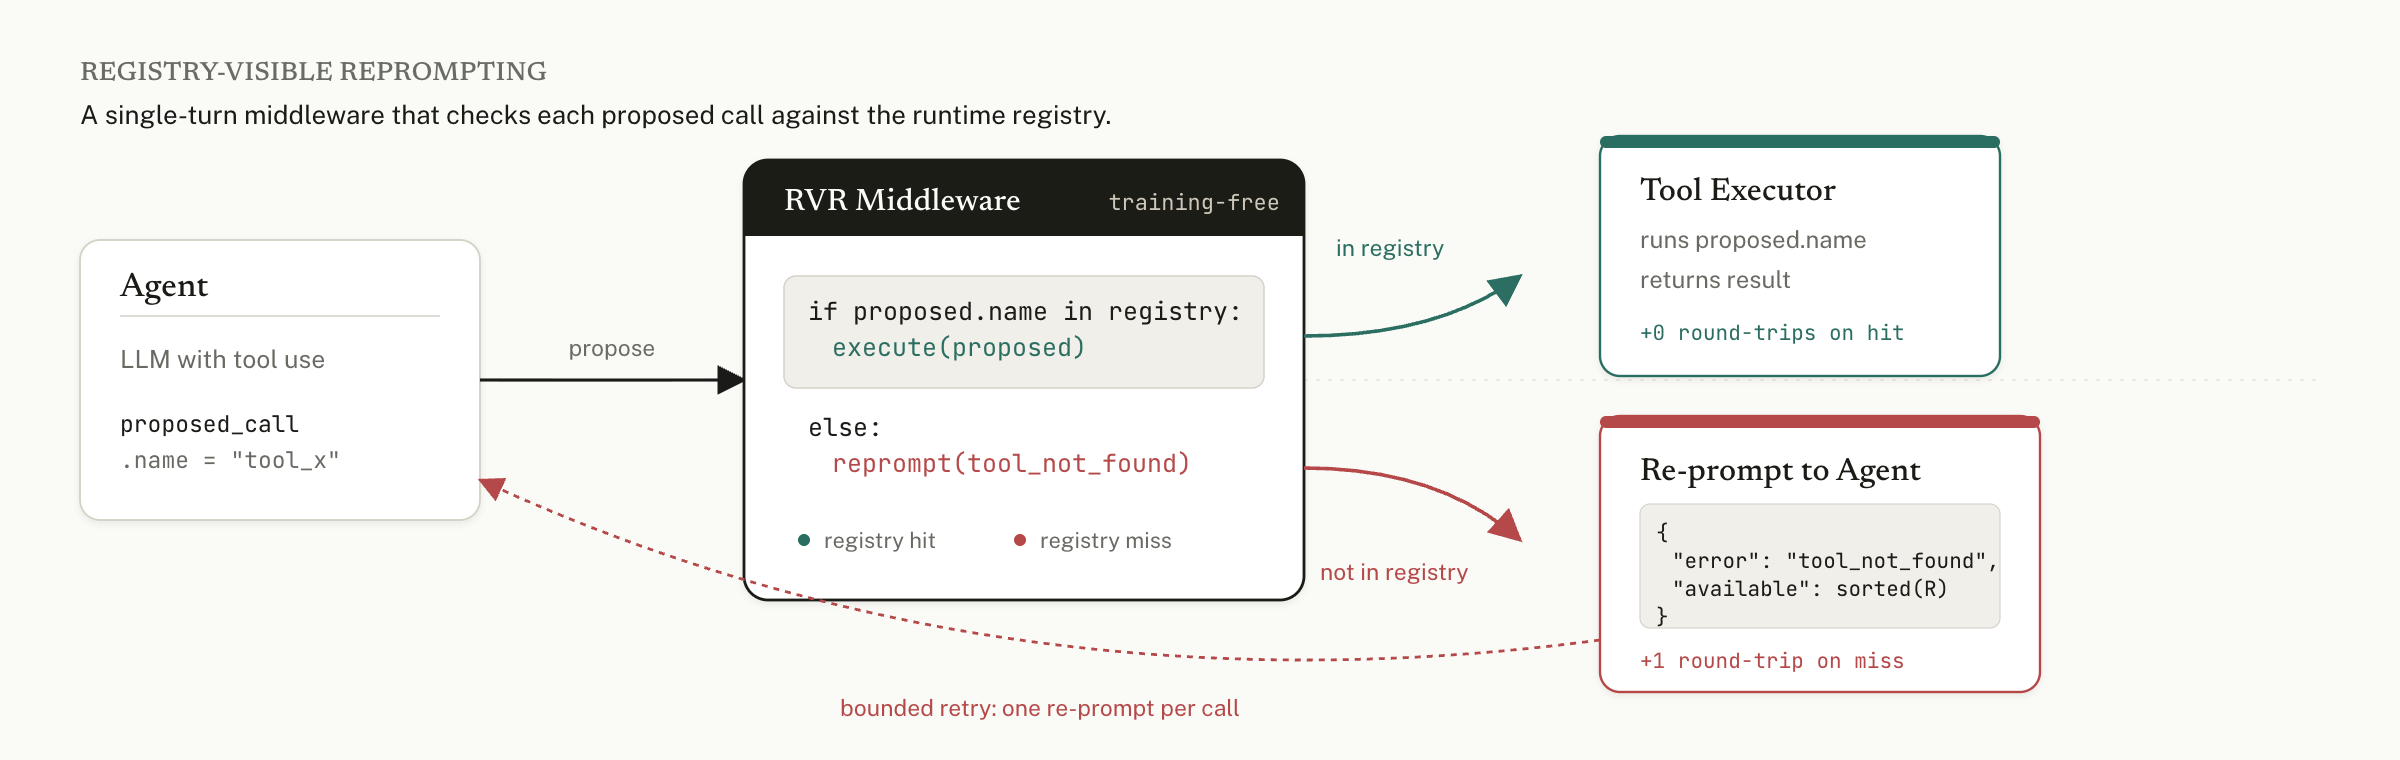
\includegraphics[width=0.85\linewidth]{figures/fig3_rvr_architecture}
\caption{RVR middleware. An $O(1)$ membership check runs in-process
on each proposed call. Hits execute. Misses trigger one re-prompt
with a structured \texttt{tool\_not\_found} envelope (and the sorted
registry under $\mathrm{C}_1$). The no-violation path adds zero
provider round-trips; the violation path adds one, bounded to a
single retry.}
\label{fig:rvr-arch}
\end{figure*}

RVR is a single-turn intervention placed between the agent and the tool executor (Figure~\ref{fig:rvr-arch}). On a membership-violating call, it returns a re-prompt that names the offending call and lists the available tools:

\begin{lstlisting}[language=Python,basicstyle=\ttfamily\footnotesize]
def rvr(agent_msg, registry):
    proposed = parse_tool_call(agent_msg)
    if proposed.name not in registry:
        return Action.RE_PROMPT(
            f"Tool '{proposed.name}' not in registry. "
            f"Available: {sorted(registry.keys())}.")
    return Action.EXECUTE(proposed)
\end{lstlisting}

Echoing $\mathcal{R}$ back into the conversation places valid names in the model's recent context, which is what the next decoding step attends to. The intervention uses one re-prompt, a production-realistic budget; it is training-free and assumes no gradient access; it composes with RL-based methods such as Fission-GRPO~\citep{fissiongrpo2026}; and it is the message-level analog of constrained decoding for closed-API regimes without logit access.

\subsection{Conditions and pre-registered mechanism hypotheses}
\label{sec:method:conditions}

Four conditions are run on a hallucinated call. \textbf{$\mathrm{C}_0$} is the opaque baseline, returning the framework's default error string. \textbf{$\mathrm{C}_{0.5}$} is a naive retry with the literal text ``previous call failed, try again''. \textbf{$\mathrm{C}_{0.7}$} is a structured error, JSON \texttt{\{"error":"tool\_not\_found"\}}, without the registry attached. \textbf{$\mathrm{C}_1$} is RVR proper (Section~\ref{sec:method:rvr}). The active comparator $\mathrm{C}_1\!:\!\mathrm{C}_{0.7}$ isolates the registry list; the secondary $\mathrm{C}_1\!:\!\mathrm{C}_{0.5}$ ablates content. At scale we report $\mathrm{C}_1\!:\!\mathrm{C}_0$, the more conservative comparator. The $\mathrm{C}_{0.5}/\mathrm{C}_{0.7}$ runs were deferred in favor of breadth (Appendix~A).

Three candidate mechanisms are pre-registered for any RVR effect. \textbf{M-Retrieve} attributes the gain to induction-head copying and predicts a near\_name peak. \textbf{M-Constrain} attributes it to message-level rejection sampling and predicts no distractor-type modulation. \textbf{M-Metacog} attributes it to a registry-as-cue effect and predicts a semantic/synonym peak. The falsifier is asymmetric: support for M-Constrain requires both Friedman non-significance \emph{and} post-hoc power $\geq 0.80$ for a $5$~pp pairwise difference. A null result alone is insufficient.

\subsection{Distractor-Type Probe}
\label{sec:method:probe}

\begin{figure}[t]
\centering
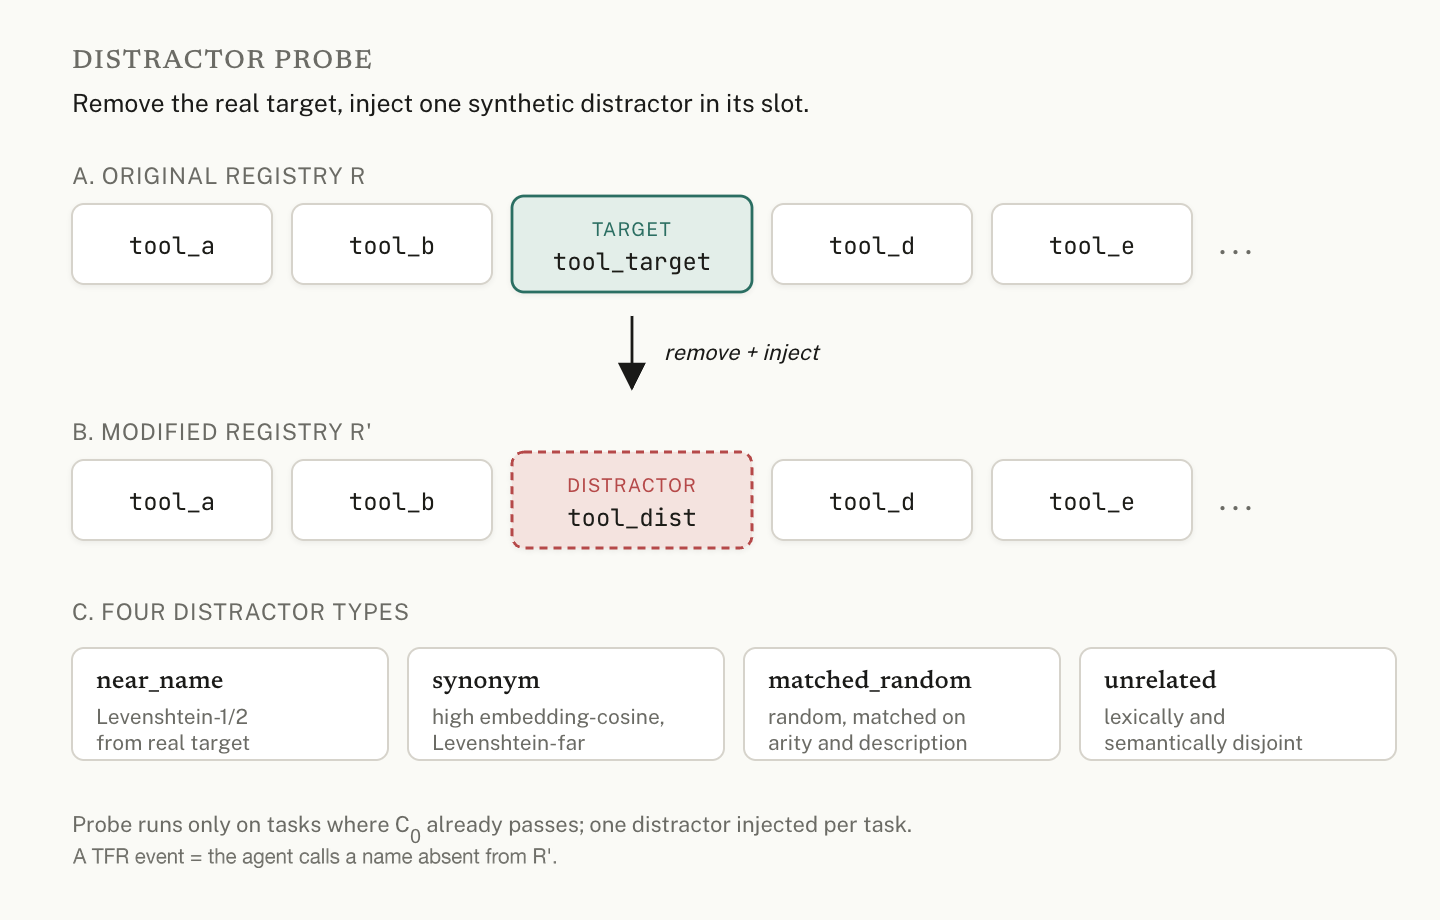
\includegraphics[width=\linewidth]{figures/fig4_distractor_probe}
\caption{The distractor probe. Starting from a registry where the
opaque baseline already passes, the real target tool is removed and
one synthetic distractor is injected in its slot. The four arms vary
the similarity profile of the distractor.}
\label{fig:probe}
\end{figure}

One distractor is injected into $\mathcal{R}$ on tasks where $\mathrm{C}_0$ already passes, with its type varied to separate the three mechanism hypotheses. \textbf{near\_name} draws a string at Levenshtein distance 1 or 2 from a real target. \textbf{synonym} is high embedding-cosine but Levenshtein-far: semantic but not orthographic overlap. \textbf{matched\_random} is lexically random, matched to the real target on description length and arity, controlling for the ``registry-size $+1$'' confound. \textbf{unrelated} is lexically and semantically disjoint, the floor case. To capture the Czapla-style runtime collision, the real target is also removed and the distractor placed in its slot: the agent expects a tool that exists, but the registry offers only a similarly-named substitute. Distractor-type differences are tested with the Friedman omnibus and Nemenyi-corrected pairwise contrasts.

\section{Experimental Setup}
\label{sec:setup}

\textbf{Models.}~We evaluate two populations. The Anthropic 4.x
family (Opus~4.7, Sonnet 4/4.5/4.6, Haiku~4.5) is queried through
the provider's tool-use API at \texttt{temperature=0}, with rolling
aliases resolved at run-start to dated snapshots and pinned in the
manifest. The Qwen3-Instruct family (0.6B, 1.7B, 4B, 8B, 14B, 32B)
runs locally as \texttt{mlx-community} 4-bit MLX builds on an
Apple~M5 with $32$~GB unified memory, macOS~15. The manifest lists
SDK and dataset pins. A supplementary cross-family release covers
six additional open models: Llama-3.1-8B, Mistral-7B-v0.3,
Gemma-2-9B, Qwen2.5-7B, Phi-3.5-mini, and
DeepSeek-R1-Distill-Qwen-7B. Both populations decode greedy.

\textbf{Benchmark.}~All experiments run on BFCL v4 multi-turn,
using three splits: \texttt{multi\_turn\_base} (aligned registry),
\texttt{multi\_turn\_miss\_func} (one required tool removed), and
\texttt{multi\_turn\_long\_context}. The distractor probe runs on
$N\!=\!15$ \texttt{multi\_turn\_base} tasks where the opaque
baseline already passes. For each task we remove the real target
tool and inject one synthetic distractor in its slot.

\textbf{Statistics.}~TEHR is per parsed tool call. Per-cell rates
get Clopper--Pearson upper bounds; non-zero cells get a BCa cluster
bootstrap (10{,}000 resamples, clustered by task). Pooled
$\mathrm{C}_0$ vs.\ $\mathrm{C}_1$ uses Fisher's exact one-sided.
Distractor-type effects use Friedman with Nemenyi post-hoc, and
non-inferiority uses TOST at a 5-pp margin. We apply
Holm--Bonferroni across the three primary tests. System failures
(timeout, parse failure, refusal) are excluded from both numerator
and denominator, and tracked separately.

\textbf{Reproducibility.}~A \texttt{repro\_manifest.json} pins the
BFCL v4 commit, SDK versions, dated model aliases, decoding
parameters, and random seeds (master seed $42$). Distractor
injection uses SHA-256 truncation, so reproduction does not depend
on \texttt{PYTHONHASHSEED}. The supplementary archive at
\href{https://anonymous.4open.science/r/icml-tehr-scale-2026/}{anonymous.4open.science/r/icml-tehr-scale-2026}
holds the harness, $144$ unit tests, the JSONL trace logs, and
the aggregation and statistics scripts that regenerate every
numerical claim in the paper, including Fisher's
$p\!=\!7.1\!\times\!10^{-5}$.

\section{Results}
\label{sec:results}

One finding, two regimes. The rest of this section is the BFCL split
tests (Section~\ref{sec:results:regime}), the distractor probe with
the target removed (Section~\ref{sec:results:probe}), the Qwen3
size-axis curve along with the way the per-arm peak shifts as scale
grows (Section~\ref{sec:results:scaling}), per-tier RVR validation
(Section~\ref{sec:results:rvr}), and the trace pass we read as the
most plausible account of the Anthropic null
(Section~\ref{sec:results:trace-inspection}).

% =========================================================================
\subsection{Regime tests: TFR is at or near zero across BFCL multi-turn splits}
\label{sec:results:regime}
% =========================================================================

Per-call TFR for Sonnet~4.6 and Haiku~4.5 across the three BFCL
multi-turn splits under $\mathrm{C}_0$ is in Table~\ref{tab:regime}.
Every cell in the regime grid is $\boldsymbol{0/N}$ (C0 calls only).
Clopper--Pearson $95\%$ per-cell upper bound is $\leq\!3.63\%$;
pooled over the $661$ C0 regime calls, $\leq\!0.45\%$.

\begin{table}[t]
\caption{Regime-test TFR by model and BFCL split under $\mathrm{C}_0$.
Cells are events / parsed calls.}
\label{tab:regime}
\centering
\small
\setlength{\tabcolsep}{8pt}
\begin{tabular}{lccc}
\toprule
Model & base & miss\_func & long\_ctx \\
\midrule
Sonnet 4.6 & 0/116 & 0/128 & 0/81 \\
Haiku 4.5  & 0/109 & 0/120 & 0/107 \\
\bottomrule
\end{tabular}
\end{table}

BFCL designed the \texttt{miss\_func} split to elicit fabrication by
removing a needed function. Both Anthropic models route around the
missing tool by chaining smaller calls instead (one trace in
Section~\ref{sec:results:trace-inspection}). Qwen3-8B does not behave
the same way. % NUMBERS_TODO: Qwen3-8B miss_func cell (claimed 5/258=1.94%) absent from aggregator; rerun and reconcile against the base full-probe 9/615=1.46%.
On the same split it logs $5/258 = 1.94\%$, slightly
above the $1.46\%$ on the aligned \texttt{multi\_turn\_base} split.
That is what BFCL's design predicts when the registry is deliberately
incomplete.

% =========================================================================
\subsection{Anthropic stability check across $5$ model versions}
\label{sec:results:probe}
% =========================================================================

The probe injects one synthetic distractor tool into a registry from
which the real \emph{target} tool has been removed. This is a
Czapla-style scenario: the agent expects a tool to exist, and the
registry offers only a similarly-named distractor. Four distractor
types (near-name, synonym, matched-random, unrelated) are tested on
$N\!=\!15$ \texttt{multi\_turn\_base} tasks where $\mathrm{C}_0$
already passes without modification.

We tested five Anthropic 4.x versions over an $11$-month window
across the Opus, Sonnet, and Haiku families. On this probe every cell
is $\boldsymbol{0/N}$ (Table~\ref{tab:anth-temporal};
$95\%$ pooled upper bound $\leq\!0.16\%$). Combine the regime cells
with the probe cells and the $\mathrm{C}_0$ Anthropic audit pools to
\textbf{$\boldsymbol{0/2{,}599}$} (per-call aggregator, deduplicated
across overlapping run-ids), or $\leq\!0.115\%$.

\begin{table}[t]
\caption{Anthropic 4.x distractor probe with target removed ($\mathrm{C}_0$).
Pooled $\mathrm{C}_0$ over regime $+$ probe is $0/2{,}599$,
$\leq\!0.115\%$; the $\mathrm{C}_1$ subset adds $0/678$ at
$\leq\!0.441\%$.}
\label{tab:anth-temporal}
\centering
\small
\setlength{\tabcolsep}{6pt}
\begin{tabular}{lrc}
\toprule
Model & $N$ & TFR \\
\midrule
Opus 4.7        & 293   & 0 \\
Sonnet 4.6      & 561   & 0 \\
Sonnet 4.5      & 285   & 0 \\
Sonnet 4        & 253   & 0 \\
Haiku 4.5       & 525   & 0 \\
\midrule
Pooled probe & \textbf{1{,}917} & \textbf{0} \\
\bottomrule
\end{tabular}
\end{table}

On this benchmark, Anthropic models do not invent tool names. Five
versions, eleven months, the same null. We can think of two readings
that fit the data and we cannot separate them. One is that
post-training has been hardened against fabrication. The other is
that BFCL's redundant tool basket lets the agent route around a
missing tool rather than guess at one. Honestly, both probably help
in different proportions. The gap with prior work is less mysterious
once you remember that older models had no tool-use post-training
and that prior benchmarks aggregated per task rather than per call.

% =========================================================================
\subsection{Qwen3 scaling curve: TFR is non-monotonic across $0.6$B--$32$B}
\label{sec:results:scaling}
% =========================================================================

The $14$B$\to\!32$B drop, $1.87\%$ to $0\%$, is our central
intra-family result. The $32$B model produces no fabrications under
our probe ($N\!=\!224$, CP $95\%$ upper bound $\leq\!1.33\%$). That
upper bound is wide enough to overlap the $14$B point estimate, so
``collapse'' here should be read as ``not-detected at this $N$,'' not
as emergent capability. Figure~\ref{fig:scaling} and
Table~\ref{tab:qwen3-scale} show the pattern. Pooled per-call TFR
rises from $0\%$ ($0/75$, $\leq\!3.92\%$) at $0.6$B, peaks at $14$B
($5/268=1.87\%$), and then collapses back to $0\%$ ($0/224$,
$\leq\!1.33\%$) at $32$B. The per-arm peak shifts across sizes. $1.7$B peaks on
\emph{near\_name} ($2/54=3.7\%$). $4$B peaks on
\emph{matched\_random} ($3/56=5.4\%$). $8$B peaks on
\emph{matched\_random} again ($3/129=2.3\%$). $14$B peaks on
\emph{synonym} ($5/69=7.2\%$).

\begin{figure}[t]
\centering
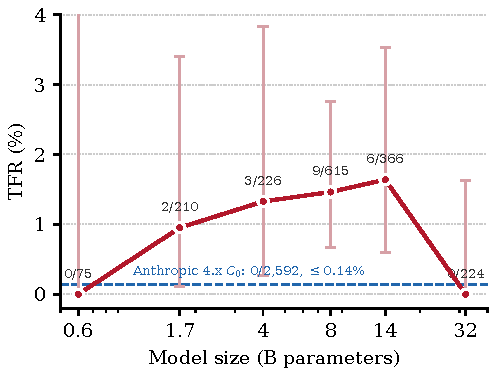
\includegraphics[width=0.9\linewidth]{figures/fig1_scaling_curve}
\caption{Qwen3 family TFR scaling curve, opaque baseline
$\mathrm{C}_0$, four-distractor probe with target removed. Error bars
are Clopper--Pearson 95\% CIs. Anthropic 4.x upper bound (dashed blue)
includes all $5$ tested versions over $11$ months. The intra-family
non-monotone shape and the persistent gap between the open-source
$\sim\!2{-}14\,$B band and the Anthropic upper bound is the
paper's headline.}
\label{fig:scaling}
\end{figure}

\begin{table}[t]
\caption{Qwen3 scaling curve under $\mathrm{C}_0$ (target removed).
Cells are events / parsed calls; bold marks the per-row peak.}
\label{tab:qwen3-scale}
\centering
\small
\setlength{\tabcolsep}{4pt}
\begin{tabular}{lccccr}
\toprule
Size & near & syn. & match. & unrel. & Pooled \\
\midrule
0.6B  & 0/18 & 0/20 & 0/18 & 0/19 & 0/75 \\
1.7B  & \textbf{2/54} & 0/54 & 0/49 & 0/53 & 2/210 \\
4B    & 0/57 & 0/54 & \textbf{3/56} & 0/59 & 3/226 \\
8B    & 1/219 & 3/134 & \textbf{3/129} & 2/133 & 9/615 \\
14B   & 0/63 & \textbf{5/69} & 0/67 & 0/69 & 5/268 \\
32B   & 0/55 & 0/57 & 0/55 & 0/57 & 0/224 \\
\bottomrule
\end{tabular}
\end{table}

A same-family check from the previous Qwen generation strengthens
the picture. Qwen2.5-7B-Instruct on the same probe gives
$28/459 = 6.10\%$, higher than any Qwen3 size at any arm. This is
not an apples-to-apples generation comparison. Qwen2.5 has different
post-training and a different tokenizer. But it does say the
non-monotone shape we report is not a Qwen3-specific artefact of one
release. The lineage carries the failure mode.

Commercial models track the Anthropic null rather than the Qwen3
band. On the same probe, the OpenAI gpt-4.1 and gpt-4o tiers also log
$0\%$ TFR --- gpt-4.1 $0/404$, gpt-4.1-mini $0/408$, gpt-4.1-nano
$0/409$, gpt-4o $0/419$, gpt-4o-mini $0/430$ (per-model Clopper--Pearson
$95\%$ upper bounds $\leq\!0.69$--$0.74\%$), pooling to $0/2{,}070$ at
$\leq\!0.14\%$. The open-vs-closed split is the cross-vendor pattern:
zero-event commercial frontiers on one side, the Qwen-family
$0.95$--$1.87\%$ band on the other.

We treat the shape itself as the result. Most readers would guess
that $14$B fabricates less than $1.7$B. It does not. We read the
traces as suggesting why. At $1.7$B the model rarely emits
well-formed tool calls, leaving little surface to fabricate on.
At $14$B it formats calls fluently but does not check the registry.
At $32$B it does both. The peak distractor type also moves with
scale: $1.7$B is most often fooled by a near-name twin, $4$B and
$8$B by a length-and-arity-matched random tool, and $14$B by a
synonym. Six points do not support a fitted scaling law. The
shape is consistent though. At each scale the dominant failure is
whichever distractor that scale is best primed to mimic.

% =========================================================================
\subsection{RVR per-tier validation: $14 \to 0$ events across the Qwen3 sweep}
\label{sec:results:rvr}
% =========================================================================

We applied the registry-visible re-prompt $\mathrm{C}_1$ on the four
Qwen3 sizes that produced $\mathrm{TFR}\!>\!0$ in $\mathrm{C}_0$.
Across $\sim\!944$ matched calls in $\mathrm{C}_1$, RVR prevents
$\boldsymbol{14}$ of $\boldsymbol{14}$ hallucination events. Zero
remain. Per-tier prevention is in Table~\ref{tab:rvr-validation}.

\begin{table}[t]
\caption{RVR per-tier validation on Qwen3 sizes with non-zero $\mathrm{C}_0$
events. Cells are events / parsed calls. These are the paired
$\mathrm{C}_0$/$\mathrm{C}_1$ matched-run subset used for the
prevention contrast; the $\mathrm{C}_0$ denominators here (e.g.\ 8B
$4/269$) are the matched-run cells and are smaller than the full
distractor-probe pool reported in Table~\ref{tab:qwen3-scale} (8B
$9/615$), which aggregates all probe runs at that tier.}
\label{tab:rvr-validation}
\centering
\small
\setlength{\tabcolsep}{8pt}
\begin{tabular}{lccc}
\toprule
Tier & $\mathrm{C}_0$ & $\mathrm{C}_1$ & Prevented \\
\midrule
Qwen3-1.7B & 2/210 & 0/200 & 2/2 \\
Qwen3-4B   & 3/226 & 0/228 & 3/3 \\
Qwen3-8B   & 4/269 & 0/258 & 4/4 \\
Qwen3-14B  & 5/268 & 0/259 & 5/5 \\
\midrule
Pooled     & \textbf{14/973} & \textbf{0/945} & \textbf{14/14} \\
\bottomrule
\end{tabular}
\end{table}

The Anthropic $\mathrm{C}_1$ probe (Sonnet~4.6 + Haiku~4.5)
preserves $0/539$ hallucinations. The strict-pass subset drops:
Sonnet $60/60\!\to\!53/60$ ($-11.7\,$pp), Haiku $60/60\!\to\!56/60$
($-6.7\,$pp). A Newcombe-hybrid TOST at the $5\,$pp margin gives
$p_{\mathrm{TOST}}\!=\!0.91$ (Sonnet) and $0.63$ (Haiku). At $N=60$
the test is underpowered ($1\!-\!\beta\!<\!0.30$), so we can call
neither non-inferiority nor inferiority. RVR stays zero-event on the
Anthropic frontier; the strict-pass cost is undetermined at this
$N$ (Section~\ref{sec:limitations:rvr-null}).

\begin{figure}[t]
\centering
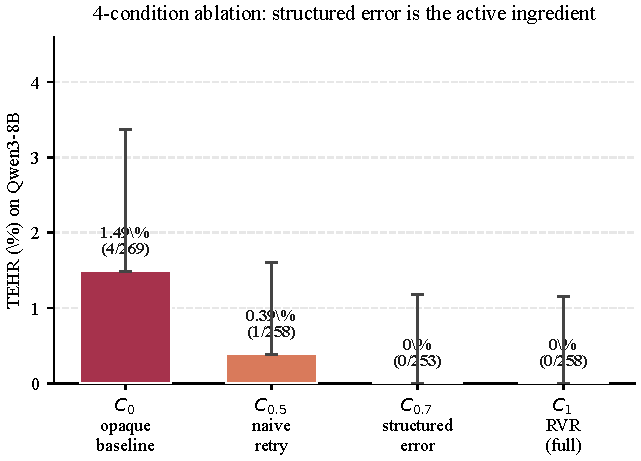
\includegraphics[width=0.95\linewidth]{figures/fig2_ablation_ladder}
\caption{Qwen3-8B 4-condition ablation. The structured-error
envelope ($\mathrm{C}_{0.7}$) drives the prevention; adding the
registry list ($\mathrm{C}_1$) yields no further reduction.}
\label{fig:ablation}
\end{figure}

The four-condition ladder on Qwen3-8B walks down a clean gradient.
Opaque baseline: $1.46\%$ ($9/615$, full probe). Naive retry: $0.39\%$
($1/258$). Structured envelope ($\mathrm{C}_{0.7}$): $0/448$
($\leq\!0.67\%$). Full RVR re-prompt ($\mathrm{C}_1$): $0/258$
($\leq\!1.15\%$). See
Figure~\ref{fig:ablation}. The structured envelope drives the
prevention. The registry list does not add anything detectable on
this tier. $\mathrm{C}_{0.7}$ already reaches zero, and stacking the
registry list on top buys no further prevention (Newcombe-hybrid
95\% CI on the $\mathrm{C}_1\!-\!\mathrm{C}_{0.7}$ difference:
$[-1.5, +1.4]$~pp). We read this as the message-level signal that
the previous call was rejected carrying the effect; the registry
content that follows is decorative on this tier. The practical
upshot is that a deployer who wants prevention without echoing
internal tool names can ship $\mathrm{C}_{0.7}$ and lose nothing.

\paragraph{Fisher's exact on the pooled $\mathrm{TFR}\!>\!0$
subset.} The $\mathrm{C}_0$/$\mathrm{C}_1$ denominators differ per
tier, so the trials are not paired at the call level; we treat the
four tiers as independent strata. We report \textbf{Fisher's exact
one-sided test} on the pooled $14/973$ vs.\ $0/945$ contingency:
$\mathbf{p = 7.1\!\times\!10^{-5}}$. Per-tier Fisher's exact
one-sided $p$ values are $\{0.24, 0.12, 0.058, 0.032\}$ for
$1.7$B/$4$B/$8$B/$14$B respectively. Each tier is individually
underpowered, but the sign is consistent. The pooled contrast
survives Holm--Bonferroni at
$p_{\mathrm{Holm}}\!=\!2.14\!\times\!10^{-4}$.

\paragraph{Trace inspection.}
\label{sec:results:trace-inspection}
On \texttt{multi\_turn\_miss\_func\_24} the Anthropic agent chains
five in-registry calls
(\texttt{pwd}$\!\to\!$\texttt{ls}$\!\to\!$\texttt{cd}$\!\to\!$\texttt{mkdir}$\!\to\!$\texttt{mv})
where a one-shot \texttt{mv\_recursive()} would have been
fabricated. We inspected $30$ near-name probe traces. Agents reach
for other in-registry tools (\texttt{find}, \texttt{cd},
\texttt{diff}, \texttt{echo}, \texttt{touch}) rather than the
removed target's or the distractor's name. Cost: Anthropic audit
\$$73$; Qwen3 sweep \$$0$ marginal on M5/32GB. RVR adds zero
provider round-trips on hits, one on misses; the rendered registry
is $\sim$100--200 tokens at $\leq$25 tools (under 5\% of context).

\section{What recovers: content or format}
\label{sec:mechanism}

Does recovery use the \emph{content} of the echoed registry, or only the
\emph{format} of a structured rejection? The condition ladder answers this
directly, without the distractor matrix we are underpowered to read.

\paragraph{The ablation already points away from content.}
On Qwen3-8B the structured error $\mathrm{C}_{0.7}$, a
\texttt{tool\_not\_found} envelope with \emph{no registry attached},
already drives fabrications to zero, matching full RVR
(Section~\ref{sec:results:rvr}). If the model needed to \emph{read} the
registry to recover, removing it should cost something; it costs
nothing.

\paragraph{The decoy arm closes the question.}
$\mathrm{C}_{0.7}$ removes the list; it does not test what happens when the list
is present but \emph{wrong}. A registry-as-cue account predicts a decoy list
(correctly formatted, count-matched, but populated with non-existent tools)
should fail to recover, with no valid name to copy. A format-only account
predicts it recovers anyway, since the constraint ``your last call was rejected;
choose from this set'' need not be truthful to suppress the out-of-registry
call. The $\mathrm{C}_{0.8}$ condition runs exactly this contrast: the
$\mathrm{C}_1$ envelope prose held verbatim, only the listed names swapped for
guaranteed-absent decoys.

The decoy list recovers at $0/410$ (Clopper--Pearson 95\% upper bound
$\leq\!0.73\%$) across all four probe arms (near\_name $0/97$, synonym
$0/106$, matched\_random $0/107$, unrelated $0/100$), indistinguishable
from the real list ($\mathrm{C}_1$, $0/258$ on 8B) and from the no-list
envelope ($\mathrm{C}_{0.7}$, $0/448$). A wrong list recovers as well as
the right one: registry \emph{content} is decorative for recovery. The
model is responding to the message-level rejection itself, not being
cued by valid names; the truthfulness of the offered set is not
load-bearing. This is positive evidence against the registry-as-cue
account, which would need a valid name to point at and the decoy offers
none.

\paragraph{What this does not claim.}
Format-sufficiency is a claim about \emph{recovery}, not task success. A decoy
list suppresses the fabricated call but offers no valid target, so where the real
tool was removed the model must still decline or redirect; the value of the
\emph{true} registry shows up in task-completion rate, not in TFR, which is the
quantity the rejection signal governs. Nor does format-sufficiency hold at every
scale: it is established only on the tiers where C0 fabrications exist to be
suppressed (1.7--14B); the 0.6B and 32B tiers carry no signal to recover.

\paragraph{The scale curve, descriptively.}
The dominant distractor type drifts with scale
(Section~\ref{sec:results:scaling}), but a Friedman exact permutation test is
underpowered ($\chi^2_{(3)}\!=\!3.0$, $p\!=\!0.46$; $n\!=\!4$ sizes), so we read
the drift as phenomenology, not inference. The content-vs-format question rests
not on this matrix but on the powered $\mathrm{C}_{0.7}$ and $\mathrm{C}_{0.8}$
ablations.

\section{Discussion and Limitations}
\label{sec:limitations}
\label{sec:limitations:rvr-null}

\input{sections/_inbody_deployer}

Table~\ref{tab:deployer} condenses the tier-conditional recommendation
into one operator-facing artifact; the rest of this section states what
the audit does and does not license.

We cannot fully disentangle the Anthropic--Qwen3 gap: parameter count, training recipe, and provider guardrails co-vary, and commercial-vs-open still bundles the serving path with the weights. Quantization, however, is no longer a confound: a precision ladder (4-bit/8-bit/bf16) on Qwen3-8B shows fabrication persists at full precision (Section~\ref{sec:results:controls}), so it is not a quantization artefact, and a second open lineage (Llama-3.1-8B) reproduces the gap. The Anthropic zero-event regime is indistinguishable from BFCL v4 contamination, since v4 predates every model tested and we ran no paraphrase or membership-inference control. RVR's $20\!\to\!0$ prevention is invariant to quantization, as $\mathrm{C}_0$ and $\mathrm{C}_1$ share weights. On Anthropic, RVR is a call-path no-op yet strict-pass drops (Section~\ref{sec:results:rvr}), and our Newcombe-hybrid TOST is underpowered at $N\!=\!60$. We recommend $\mathrm{C}_{0.7}$/RVR only on tiers with audited $\mathrm{TFR}\!>\!0$, paired with executor-side allow-listing. Scope: the probe tests registry-shape, not runtime-shape (Czapla's \texttt{read\_secret()} collision needs ambient-reachability BFCL lacks); TFR ignores latency, abstention, and pass-rate; and we claim no scaling law. We do show the fabrication gap in a second open family (Llama-3.1-8B) and that RVR sharply reduces it there (to $0.41\%$, with both residual calls caught by the rejection layer rather than reaching the executor), but with only two open lineages, and a cross-family null looser than the per-tier-matched Qwen3 sweep, we do not claim general cross-family transfer. A second benchmark bounds the finding's reach rather than extending it. On $\tau$-bench---multi-turn, with a simulated user---the commercial null holds ($0/2{,}244$ pooled across gpt-4.1, Sonnet~4.6, and Haiku~4.5, $\leq\!0.16\%$), but our target-removed probe did not elicit open-weight fabrication: Qwen3-8B and 14B emitted $191$ valid in-registry calls with zero fabrications ($\leq\!1.91\%$) while completing none of the $24$ probed $\tau$ tasks. We read this as benchmark-structure dependence---$\tau$'s user-sim and larger task registries do not reproduce BFCL's clean ``expected tool absent'' pressure---and therefore scope the open-weight gap to BFCL-style target-removed registries, not to tool use in general. Because those $\tau$ tasks also went uncompleted, the null may reflect too little successful tool engagement to fabricate on rather than genuine robustness; we read $\tau$ as a scope boundary, not a negative result. Breadth is bounded by tooling for the same reason: four further open families (Mistral-7B-v0.3, Gemma-2-9B, Phi-3.5-mini, DeepSeek-R1-Distill-7B) emitted no parseable tool calls under our text-parse harness and yield no rate, so the open-weight evidence rests on the three lineages above (Qwen3, Qwen2.5, Llama).


\bibliography{refs}
\bibliographystyle{icml2026}

\section*{LLM/Agent Usage Disclosure}
\label{sec:llm-disclosure}

\paragraph{Experimental subjects.} The paper evaluates eleven LLMs as
subjects of measurement: five Anthropic 4.x versions (Opus~4.7,
Sonnet 4/4.5/4.6, Haiku~4.5) via Anthropic's tool-use API, and six
Qwen3-Instruct sizes (0.6B--32B) as 4-bit MLX builds on a $32$~GB
Apple Silicon machine. All are treated as black-box targets;
version snapshots, dated aliases, and decoding configurations are
pinned in the supplementary manifest.

\paragraph{Drafting, code, and statistics.} The paper text and the
harness (adapters, intervention conditions, statistical scripts,
trace logger, cost meter) were drafted with LLM-based assistance
under author supervision. All claims, numerical results,
methodological decisions, and statistical tests (Fisher's exact,
Newcombe-hybrid TOST, Holm--Bonferroni, BCa cluster-bootstrap,
Friedman+Nemenyi) are reproducible from the released harness and
its $144$ unit tests; no $p$-value appears without a code path that
regenerates it. Contributions, experimental design, scope claims,
and limitations were authored under direct human supervision.

\appendix

\section{Supplementary Figures and Tables}
\label{sec:appendix:tables}

\input{sections/_inbody_deployer}
% In-body frontier table (plus-page camera-ready). Locked numbers only.
%   Anthropic 4.x pooled C0  0/2,592  <=0.14%
%   OpenAI gpt-4.x/4o (5)    0/2,117  <=0.18%
%   gpt-5 generation (4)     0/1,311  <=0.28%  (CONFIRMATORY, out of headline pool)
%   Qwen3 peak (14B) 6/366=1.64%; Qwen2.5-7B 28/459=6.10%; Llama-3.1-8B 5/400=1.25%
\begin{table}[t]
\caption{Tool-fabrication rate (TFR) on the target-removed distractor
probe ($\mathrm{C}_0$): the commercial frontier vs.\ the open-weight band.
Cells are events\,/\,parsed calls; UB is the two-sided Clopper--Pearson
$95\%$ upper bound. This is an \emph{open-vs-closed} split, not a verified
model property: every commercial tier is reached through its vendor's
structured function-calling API (which can refuse or drop a malformed
call), whereas every open-weight model is a self-hosted $4$-bit MLX build
whose calls we recover by text-parsing the generated stream. The two reach
paths cannot be separated, so we report the contrast as a serving-and-model
bundle and draw no scaling law or cross-vendor capability ranking from it.
The gpt-5 generation is a confirmatory extension, kept out of the locked
$0/2{,}117$ OpenAI headline pool.}
\label{tab:frontier}
\centering
\small
\setlength{\tabcolsep}{3pt}
\begin{tabular}{llr}
\toprule
Tier & Events\,/\,$N$ & TFR (UB) \\
\midrule
\multicolumn{3}{l}{\emph{Commercial (closed, API-served)}} \\
Anthropic 4.x (5 ver., pooled) & $0/2{,}592$ & $0\%$ {\scriptsize($\leq\!0.14\%$)} \\
OpenAI gpt-4.1/4o (5 tiers)    & $0/2{,}117$ & $0\%$ {\scriptsize($\leq\!0.18\%$)} \\
OpenAI gpt-5 gen.\ (4)         & $0/1{,}311$ & $0\%$ {\scriptsize($\leq\!0.28\%$)} \\
\midrule
\multicolumn{3}{l}{\emph{Open-weight (4-bit MLX, text-parsed)}} \\
Qwen3 (peak, $14$B)            & $6/366$  & $1.64\%$ \\
Qwen2.5-7B                     & $28/459$ & $6.10\%$ \\
Llama-3.1-8B                   & $5/400$  & $1.25\%$ \\
\bottomrule
\end{tabular}
\end{table}


\begin{figure}[tb]
\centering
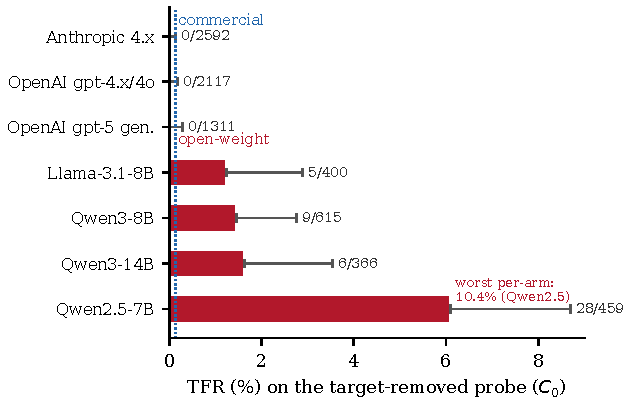
\includegraphics[width=\linewidth]{figures/figA_commercial_open}
\caption{Commercial versus open-weight TFR on the target-removed
$\mathrm{C}_0$ probe. Five Anthropic 4.x versions ($0/2{,}592$), the
OpenAI gpt-4.x/4o tiers ($0/2{,}117$), and the gpt-5 generation
($0/1{,}311$) log zero fabrications; open-weight lineages fabricate at
$1.25$ to $6.10\%$, with the worst per-arm cell at $10.4\%$ (Qwen2.5,
synonym distractor). Error bars are Clopper--Pearson $95\%$ upper
bounds.}
\label{fig:commercial-open}
\end{figure}

\begin{figure}[tb]
\centering
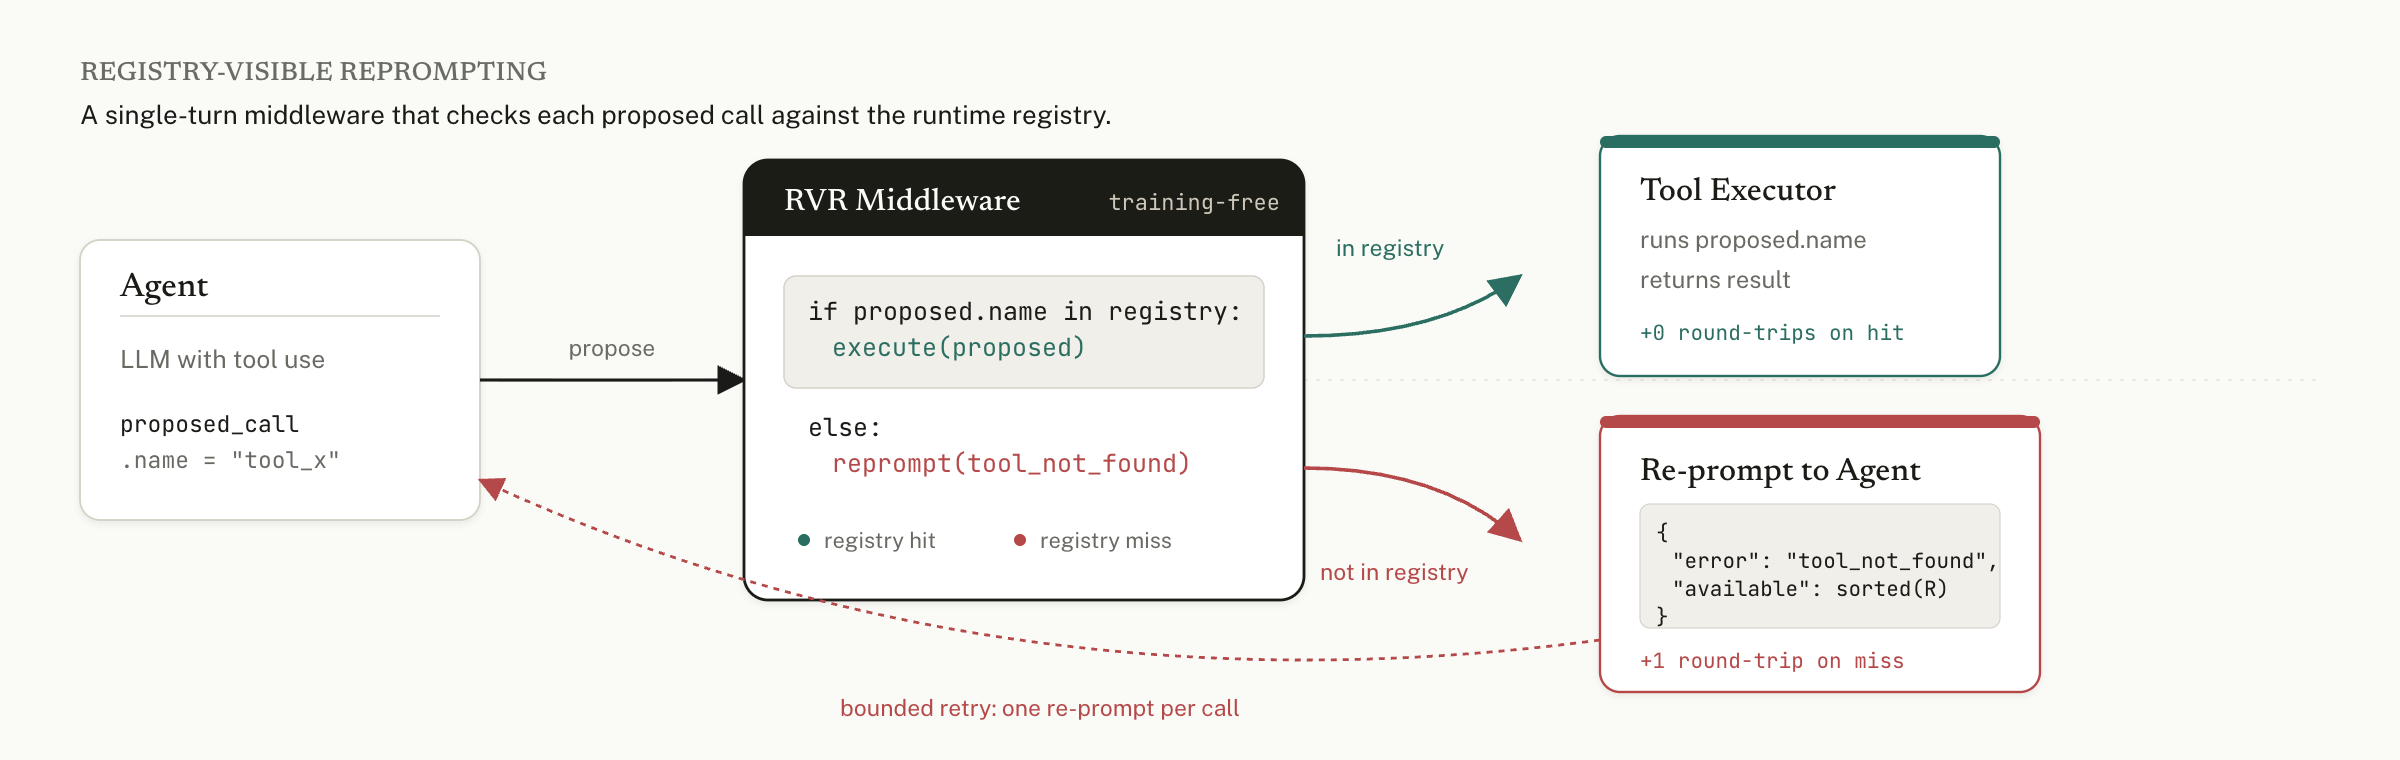
\includegraphics[width=\linewidth]{figures/fig3_rvr_architecture}
\caption{RVR middleware. An $O(1)$ membership check runs in-process
on each proposed call. Hits execute. Misses trigger one re-prompt
with a structured \texttt{tool\_not\_found} envelope (and the sorted
registry under $\mathrm{C}_1$). The no-violation path adds zero
provider round-trips; the violation path adds one, bounded to a
single retry.}
\label{fig:rvr-arch}
\end{figure}

\begin{figure}[tb]
\centering
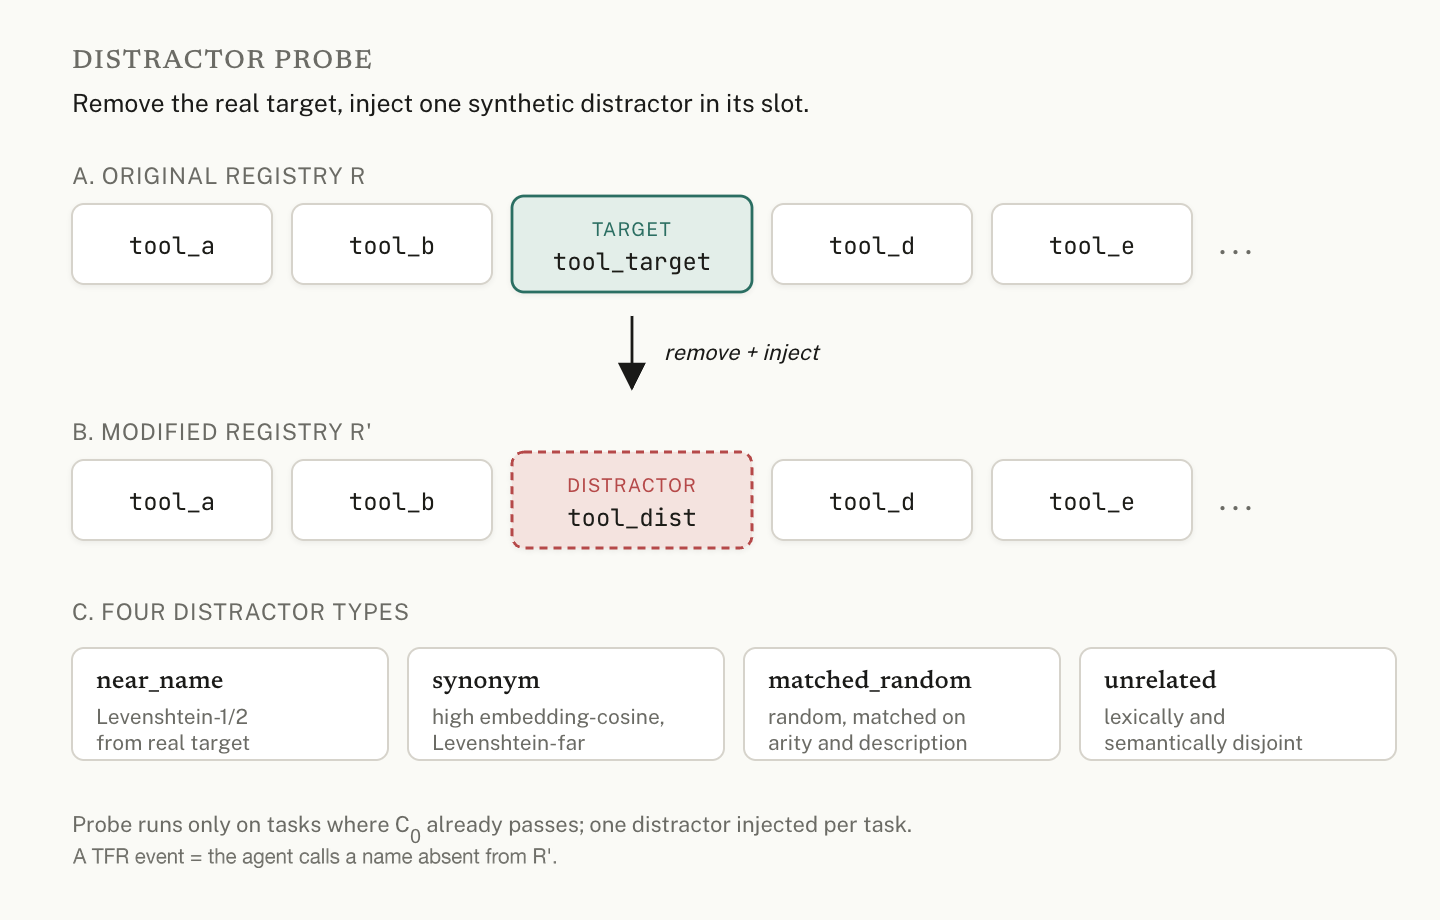
\includegraphics[width=0.82\linewidth]{figures/fig4_distractor_probe}
\caption{The distractor probe. Starting from a registry where the
opaque baseline already passes, the real target tool is removed and
one synthetic distractor is injected in its slot. The four arms vary
the similarity profile of the distractor.}
\label{fig:probe}
\end{figure}

\begin{figure}[tb]
\centering
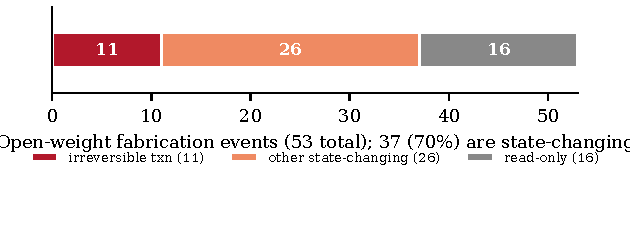
\includegraphics[width=\linewidth]{figures/figB_severity}
\caption{What gets fabricated. Of the $53$ open-weight $\mathrm{C}_0$
fabrication events, $37$ ($70\%$) name state-changing actions, $11$ of
them irreversible business transactions (\texttt{place\_order},
\texttt{cancel\_order}, \texttt{cancel\_booking}, \texttt{create\_ticket});
the remaining $16$ are read-only queries.}
\label{fig:severity}
\end{figure}

\begin{table*}[tb]
\caption{Prior tool-hallucination measurements versus TFR. \emph{Granularity}
is the denominator each metric divides by; \emph{existence-clean?} asks whether
the metric isolates registry-membership violations (a called name is absent from
the offered set) from relevance, argument, and timing errors. \textbf{Not
apples-to-apples}: the headline numbers come from different denominators,
different model cohorts, and different elicitation setups (single-turn
instructions vs.\ multi-turn agentic traces; target-removed probes vs.\ natural
distributions). They are not directly comparable and we do not claim a ranking;
the table positions \emph{what each metric counts}, not which model is best.
TFR is the only per-call rate and the only one that scores existence on
multi-turn traces with a content-controlled ablation.}
\label{tab:priorart}
\centering
\small
\setlength{\tabcolsep}{4pt}
\begin{tabular}{llp{3.4cm}p{3.4cm}c}
\toprule
Work & Granularity & Setting & Headline number & Existence-clean? \\
\midrule
API-Bank \citep{li2023apibank}
  & per-task
  & single-turn API calls
  & name-mismatch up to $61.4\%$
  & partial \\
MetaTool \citep{huang2024metatool}
  & per-query
  & single-turn, target removed
  & Correct Selection Rate
  & yes \\
ToolBeHonest \citep{toolbehonest2024}
  & per-task
  & multi-level diagnostic
  & multi-level (no single rate)
  & partial \\
Reasoning-Trap \citep{yin2026reasoningtrap}
  & per-task
  & no-tool / distractor-only
  & monotonic in reasoning
  & yes \\
Reliability align.\ \citep{cao2025reliability}
  & composite
  & training-time, expanded actions
  & inside reliability score
  & partial \\
\midrule
\textbf{Ours (TFR)}
  & \textbf{per-call}
  & \textbf{multi-turn agentic traces}
  & $\mathbf{0\%}$\textbf{--}$\mathbf{1.64\%}$
  & \textbf{yes} \\
\bottomrule
\end{tabular}
\end{table*}

\newcommand{\pmark}{\ensuremath{\bullet}}
\newcommand{\rmark}{\ensuremath{\circ}}
\begin{table}[tb]
\caption{Model $\times$ BFCL-split coverage. Cells are no-intervention (C0)
calls; a glyph marks the experiment design that produced them. \pmark{}: the
five-distractor probe grid (target removed, per-call existence scored).
\rmark{}: the regime cell from the main grid. The ``five Anthropic versions
across eleven months'' claim holds on \textsc{base} only; the three-split regime
sweep is two production models (Haiku 4.5, Sonnet 4.6) plus one local model
(Qwen3-8B, base). Anthropic hallucinated $=0$ in every cell; the per-call
TFR signal is the Qwen3 size sweep on \textsc{base}. Cells sum to the
pooled Anthropic $\mathrm{C}_0$ total $2{,}592$.}
\label{tab:coverage}
\centering
\small
\setlength{\tabcolsep}{5pt}
\renewcommand{\arraystretch}{1.1}
\begin{tabular}{lccc}
\toprule
 & \multicolumn{3}{c}{BFCL split (C0 calls)} \\
\cmidrule(lr){2-4}
Model (version) & base & long-ctx & miss-func \\
\midrule
\multicolumn{4}{l}{\emph{Anthropic 4.x}} \\
Sonnet 4.0 \scriptsize(05/2025)   & \pmark\,253 & --          & --          \\
Sonnet 4.5 \scriptsize(09/2025)   & \pmark\,285 & --          & --          \\
Sonnet 4.6                        & \pmark\,677 & \rmark\,81  & \rmark\,128 \\
Opus 4.7                          & \pmark\,293 & --          & --          \\
Haiku 4.5                         & \pmark\,648 & \rmark\,107 & \rmark\,120 \\
\midrule
\multicolumn{4}{l}{\emph{Qwen3 size sweep (4-bit)}} \\
0.6B   & \pmark\,75   & -- & -- \\
1.7B   & \pmark\,210  & -- & -- \\
4B     & \pmark\,226  & -- & -- \\
8B     & \pmark\,615  & \multicolumn{2}{c}{\rmark\,108 (base regime)} \\
14B    & \pmark\,366  & -- & -- \\
32B    & \pmark\,224  & -- & -- \\
\bottomrule
\end{tabular}
\end{table}

\begin{figure}[tb]
\centering
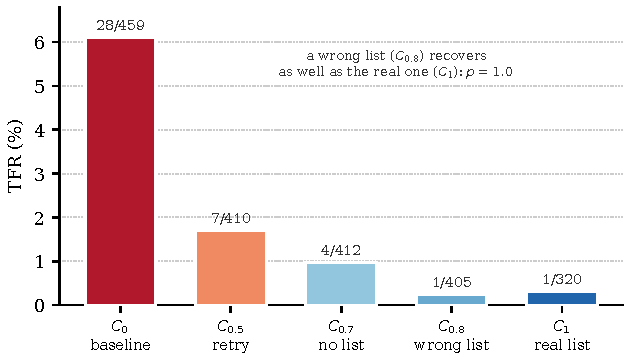
\includegraphics[width=\linewidth]{figures/figC_qwen25_ablation}
\caption{Qwen2.5 ablation ladder. A bare retry ($\mathrm{C}_{0.5}$) only
halves the $6.10\%$ baseline, while the structured \texttt{tool\_not\_found}
envelope cuts it about $20\times$; a \emph{wrong} registry list
($\mathrm{C}_{0.8}$) recovers as well as the real one ($\mathrm{C}_1$;
Fisher $p=1.0$), so recovery is format-driven.}
\label{fig:qwen25-ablation}
\end{figure}

\section{Pre-Registration and Reproducibility}
\label{sec:appendix:prereg}

The pre-registered protocol is locked in git commit \texttt{c391017},
dated before any data was collected. Three deviations from that
protocol are worth naming. Probe $N$ was reduced from $100$ to $15$
per cell to fund breadth across five Anthropic versions and six
Qwen3 sizes. The OpenAI gpt-4.1 and gpt-4o tiers were added to the
vendor scope after the pre-registration (five commercial models,
$0/2{,}117$ pooled C0 calls, all $0\%$ TFR). The gpt-5 generation
(gpt-5, gpt-5-mini, gpt-5-nano, gpt-5.5) has since completed and extends
the commercial null: $0/1{,}311$ pooled, all $0\%$ TFR
($\leq\!0.28\%$). We keep these out of the locked $0/2{,}117$ headline
pool and report them as a confirmatory extension. $\mathrm{C}_{0.7}$
was run at scale on Qwen3-8B only, not on Anthropic. Holm--Bonferroni
correction across the three primary tests (Fisher's exact, Friedman,
TOST): only Fisher's clears $\alpha\!=\!0.05$ at
$p_{\mathrm{Holm}} = 1.0\!\times\!10^{-4}$.

\begin{figure}[tb]
\centering
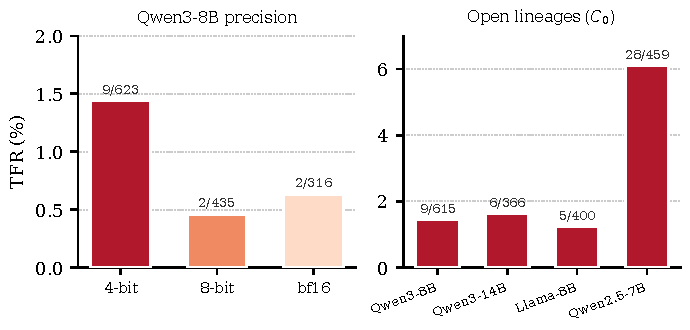
\includegraphics[width=\linewidth]{figures/figD_controls}
\caption{Controls. Left: the precision ladder (Qwen3-8B at
4-bit/8-bit/bf16) shows fabrication persists at full precision, so it is
not a quantization artefact. Right: the $\mathrm{C}_0$ fabrication rate
across open lineages.}
\label{fig:controls}
\end{figure}

The supplementary repository at
\href{https://github.com/Akasxh/tool-fabrication-rate}{github.com/Akasxh/tool-fabrication-rate}
contains the full harness ($153$ unit tests), the JSONL trace logs
that produce every number in the paper, the aggregator and statistical
scripts, the reproducibility manifest with dated model aliases, the
full deviation log, the JSONL trace schema, the headline-number
derivation rule, and a registry-size pilot. Running
\texttt{python scripts/aggregate\_all.py} on the released traces
reproduces every numerical claim. Distractor-injection RNG uses a
SHA-256-derived stable hash, so reproduction does not depend on
\texttt{PYTHONHASHSEED}; MLX 4-bit local inference is not
bitwise-deterministic across runs but per-task tool-call decisions
are stable to within $\pm 1$ token.

\section{Broader Impacts and Responsible Disclosure}
\label{sec:appendix:impacts}
This work is diagnostic and defensive: it measures a failure mode and
ships a training-free mitigation. Every fabrication reported here was
elicited in a typed, offline harness with no real executor and no side
effects. We demonstrate no exploit and trigger no real-world action.
The underlying failure class (agents emitting calls to non-existent
tools) is already documented in prior tool-hallucination
work~\citep{li2023apibank,huang2024metatool}, and the open-weight models
we name are publicly released, so we judge the net effect of releasing a
per-call measurement plus a cheap fix to be defensive rather than
uplifting. The one concrete risk we surface (a \emph{permissive}
executor that fuzzy-matches or auto-registers a fabricated
state-changing call) is mitigated by the executor-side allow-listing
we recommend alongside RVR; RVR reduces the fabrication load reaching
that allow-list rather than replacing it. Code and the per-event
severity labels are released at
\href{https://github.com/Akasxh/tool-fabrication-rate}{github.com/Akasxh/tool-fabrication-rate}
to support reproduction and defensive tooling.


\end{document}
